\subsection{Features}

In this work we want to find \emph{primitive} features, resembling the possible types of strokes used to write a word, to characterize the sample from which they are extracted in order to perform clustering on their set.

The features are identified by the study of a sub-portion, or window, of the images extracted by the paper on which this work is based.

The features are located through a study of an area, the window, with which they are implicitly associated: as such there is no clear order of which of the possibly multiple features found in the area comes first.
Due to the absence of such \emph{native} order the string that defines a window is maintained consistent with the other strings trough the convention of generating the string with the features' identifiers always taking the same order, if present.

The chosen way to resolve the issue however presents the problem of making sliding windows inapplicable: this means that a sample must necessarily be cut in separate windows, which are allowed to overlap, with the corresponding effect that due to the random cut some features like \textit{loops} may not be recognised in an instance and recognised in another. 

Each sample is associated to a characterizing string of characters made from the identifiers of the features recognized in the sample.
The string is constructed modularly by appending in order the strings associated to each window the sample is divided in.
After having recognised the presence of a feature in a given window the corresponding identifier is added to the end of the string correspondent to the window; the order in which the features are searched and thus added to the queue is decided a priori and maintained consistent during the construction of the strings. 


\paragraph{Windows}

Currently we have chosen to cut the samples in windows of 32 pixels each, with the exception of the last part of the sample that, deemed irrelevant to the end of characterization due to containing almost always white space, is simply ignored.

These windows are spaced only 16 pixels from the preceding and succeeding one, with the intent of creating overlap and lengthening the string that characterizes the samples.

While the simplest way to create the windows is simply creating a new PIX with the required coordinates it requires unnecessary passages and time in the creation of new objects. We have thus preferred to increase the complexity of the functions that search for the features, to whom we pass as a variable the original sample PIX with information about the \textit{offset} at which to start the search and the \textit{width} of the window. The width of the window passed has actually a non banal meaning duo to the fact that different features are linked to areas of the image with varying dimensions: for example we can't reasonably search for an horizontal line and a vertical line utilizing windows with the same width due to the fact that horizontal lines realistically will require windows with great width but will not have requisites on the height.
The height of the windows used is never considered as a parameter since for all features' functions the height is customarily the whole height of the sample.  


//possibilmente sezione stringa/caratteri?

\subsubsection{Whitespace}  

The first feature that is search in the windows is the white space. This way if a window is identified as blank will not be necessary to proceed with the investigation of other features, saving time.

A window is identified as blank if the average pixel values is below a preset white threshold.

\subsubsection{Loop}

The feature that represents a loop is recognized only with maximum window size.
To locate a loop is initially found a black pixel. The idea behind is to imagine that we had found a point on the border and meet two transitions going in the same direction, first from black to white then from white to black. Between the two transitions there must be a minimum step above a preset threshold where the pixels are white.

If the above condition occurs then we verify that it is real in the same way along the horizontal axis. We then sit in the center of the loop (the median value of the segment described above) and check that, moving both right or left you get a transition from white to black after a suitable number of white pixels.

The implemented method has numerous problems related mainly to the identification of the center of the loop in the segment. With a value of threshold too high also might have to discard some loops too small. The method also does not take into account the thickness of the stroke.
However, with appropriate threshold values you can get good results and to identify obvious loops of various segments.

\subsubsection{Dot}

To search for Dots within the segment we first proceed locating the \emph{connected components} inside it. The individual components are extracted and inserted into a \emph{box} which we can know the size and the relative position to the segment.

At this point we look for those boxes with dimensions between two preset values (minimum and maximum radius) and those that meet this condition are most likely points.

Using connected components we can retrieve Dot feature in a simple way.

\subsubsection{Diagonal line}

The feature representing a diagonal line, both upward and downward facing, is extracted through a simple exhaustive scansion of the window for lines of connected black pixels that have an incline in a range of values and are sufficiently long.

At the moment the function doesn't account for the width of the lines found, thus diagonal features can be recognised in a shapeless blob of black pixel that is sufficiently big. 
   
There's a distinction for diagonal features that appear in the lower and upper bottom of the window.
At most in a window the function identifies a couple of upward and a couple of downward facing lines (lower and upper parts), once one has been found it stops searching for the same type.

\subsubsection{Cross}
The function, having found at most a lower and upper case for upward and downward diagonal lines, proceeds to confront the edge points of these lines: if they possibly intersects it extracts a \emph{crossing} feature with distinction if the crossing happens in the lower or upper part of the window. 

The problems with this sub-feature are that intersections of bottom and upper lines of the same type (e.g. both upward facing) with different inclines are not recognised, in the same way there's no consideration for intersections made from lines that are not the "primary" bottom and upper diagonals: if in a single windows are present more lower upwards diagonals and one of them other than the first intersects the recognised downward diagonal, such a crossing is ignored.

The crossing feature may also not necessarily be a complete intersection, in fact for recognition there just needs to be a merging of a downward and upward line. 


\subsubsection{Horizontal and Vertical line}
Both horizontal and vertical lines' features are extracted through
a simple scan of the window.
The horizontal lines requires a double-window for their implicit characteristic.
The function identifies a line if it finds a connected row or column of black pixels that has sufficient length, in particular it distinguishes the lines found in normal or long through an ulterior threshold.
Once a fitting line has been found the function keeps searching for more, continuing the scansion of the window after having moved a certain distance from the last line found in order not to confuse a particularly thick stroke as different separate lines.
There still persists the problem that the stroke width is not fully considered so a big blob of black pixels is seen as a series of horizontal and vertical lines, at the same time such an occurrence is rare so the presence of many horizontal and vertical lines ends up distinguishing the word in itself.    

\subsection{Feature extraction example}

We present now an example of extraction of features from a word. We initially create, as described above, a sliding window that scrolls along the image by a fixed step. Than, for each section,  features are extracted and a substring is generated.

\begin{figure}[!ht]
\centering
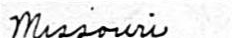
\includegraphics[width=0.5\textwidth]{images/missiouri/missiouri.jpg}
\caption{Feature extraction from \emph{Missiouri} word}
\label{fig:ap}
\end{figure} 

\begin{figure}[!ht]
 \centering
 \subfigure[]
   {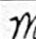
\includegraphics[width=0.06\textwidth]{images/missiouri/0.jpg}}
 \subfigure[]
   {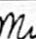
\includegraphics[width=0.06\textwidth]{images/missiouri/1.jpg}}
 \subfigure[]
   {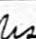
\includegraphics[width=0.06\textwidth]{images/missiouri/2.jpg}}
 \subfigure[]
   {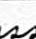
\includegraphics[width=0.06\textwidth]{images/missiouri/3.jpg}}
 \subfigure[]
   {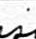
\includegraphics[width=0.06\textwidth]{images/missiouri/4.jpg}}
 \subfigure[]
   {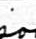
\includegraphics[width=0.06\textwidth]{images/missiouri/5.jpg}}
 \subfigure[]
   {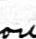
\includegraphics[width=0.06\textwidth]{images/missiouri/6.jpg}}
 \subfigure[]
   {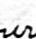
\includegraphics[width=0.06\textwidth]{images/missiouri/7.jpg}}
 \subfigure[]
   {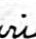
\includegraphics[width=0.06\textwidth]{images/missiouri/8.jpg}}  
 \subfigure[]
   {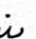
\includegraphics[width=0.06\textwidth]{images/missiouri/9.jpg}}
 \subfigure[]
   {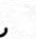
\includegraphics[width=0.06\textwidth]{images/missiouri/10.jpg}}
 \subfigure[]
   {
\includegraphics[width=0.06\textwidth]{images/missiouri/11.png}}
 \subfigure[]
   {
\includegraphics[width=0.06\textwidth]{images/missiouri/12.png}}   
 \caption{Sliding window segmentation}
 \end{figure}

\begin{enumerate}[label=(\alph*)]
\item Some \textbf{diagonal lines} (ascending (s) and descending (u) ), at the top (S) and at the bottom (s) of the image. Generated string: ''\emph{sSUusSUSu}''.
\item As the previous image and two more diagonal lines representing the "\emph{i}". An \textbf{horizonal line} (H). Generated string: ''\emph{sSUusSUSuHsu}''.
\item Some diagonal lines and, at the end of the window, an horizontal line. Generated string: ''\emph{ssSusSsH}''.
\item Two consecutive similar character represented by diagonal lines and \textbf{vertical lines} in the middle. Generated string: ''\emph{sVHsV}''.
\item In that window we can find a \textbf{dot} (.). Generated string: ''\emph{ssVHs.}''
\item The same previous dot and a little \textbf{loop} (L) at the bottom. Generated string: ''\emph{ssVs.LssH}''.
\item The same loop as previous, an horizontal line a vertical line and two diagonal. Generated string: ''\emph{LVHssu}''.
\item Generated string: ''\emph{ssVHus}''.
\item The other dot here. Generated string ''\emph{ssus.H}''.
\item An i. Generated string: ''\emph{ssuu.}''.
\item Only a diagonal line. Generated string: ''\emph{s}''.
\item Empty window.
\item Empty window.
\end{enumerate}

Once those strings are generated they are combined together to generate the word \textit{structure string}. 